\documentclass{beamer}
\usetheme{metropolis}           % Use metropolis theme
% additional config
\usepackage[at]{easylist} % list utility
\usepackage{booktabs} % table toprule, midrule, bottomrule
\usepackage[utf8]{inputenc}
\usepackage{listings}
\usepackage{xcolor}
\usepackage{color}
%\usepackage{subfig}
\usepackage{bm}
\usepackage{subfigure}
\graphicspath{{figures/}}
% colors define
\definecolor{pblue}{rgb}{0.13,0.13,1}
\definecolor{pgreen}{rgb}{0,0.5,0}
\definecolor{pred}{rgb}{0.9,0,0}
\definecolor{pgrey}{rgb}{0.46,0.45,0.48}
\definecolor{RoyalBlue}{rgb}{0.254902,0.411765,0.882353}
\definecolor{lightgray}{rgb}{.9,.9,.9}
\definecolor{darkgray}{rgb}{.4,.4,.4}
\definecolor{purple}{rgb}{0.65, 0.12, 0.82}

\lstdefinelanguage{JavaScript}{
  keywords={typeof, new, true, false, catch, function, return, null, catch, switch, var, if, in, while, do, else, case, break},
  keywordstyle=\color{pred}\bfseries,
  ndkeywords={class, export, boolean, throw, implements, import, this},
  ndkeywordstyle=\color{pgrey}\bfseries,
  identifierstyle=\color{black},
  sensitive=false,
  comment=[l]{//},
  morecomment=[s]{/*}{*/},
  commentstyle=\color{purple}\ttfamily,
  stringstyle=\color{pblue}\ttfamily,
  morestring=[b]',
  morestring=[b]"
}

\lstset{
   language=JavaScript,
   backgroundcolor=\color{lightgray},
   extendedchars=true,
   basicstyle=\footnotesize\ttfamily,
   showstringspaces=false,
   showspaces=false,
   numbers=left,
   numberstyle=\footnotesize,
   numbersep=9pt,
   tabsize=2,
   breaklines=true,
   showtabs=false,
   captionpos=b
}

\title{Deep Learning and TensorFlow}
\date{\today}
\author{Dapeng Hu, Qinglong Tian, Haozhe Zhang, Min Zhang}
\institute{STAT 580 Statistical Computing\\Department of Statistics\\ Iowa State University}

\setbeamertemplate{blocks}[default]

\begin{document}
\maketitle

\begin{frame}
	\begin{figure}
		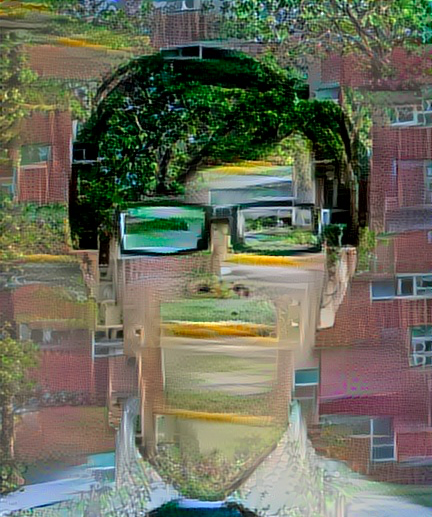
\includegraphics[width=0.59\linewidth]{style_transfer.png}
	\end{figure}
	
\end{frame}

\begin{frame}
\frametitle{Content}
\setbeamertemplate{section in toc}[sections numbered]
\tableofcontents[hideallsubsections]
\end{frame}


\section{Why Deep Learning?}
\begin{frame}
	\frametitle{More Hidden Layers?}
	\begin{itemize}
		\item The signal is getting weaker
\item Non-convex problem
\item Slow Convergence
\item Weakness of Gradient Descent: Local Optima
	\end{itemize}
\end{frame}

\begin{frame}
	\frametitle{Breakthrough}
	{\small Hinton, G. E., \& Salakhutdinov, R. R. (2006). Reducing the dimensionality of data with neural networks. science, 313(5786), 504-507.}
	\begin{figure}
		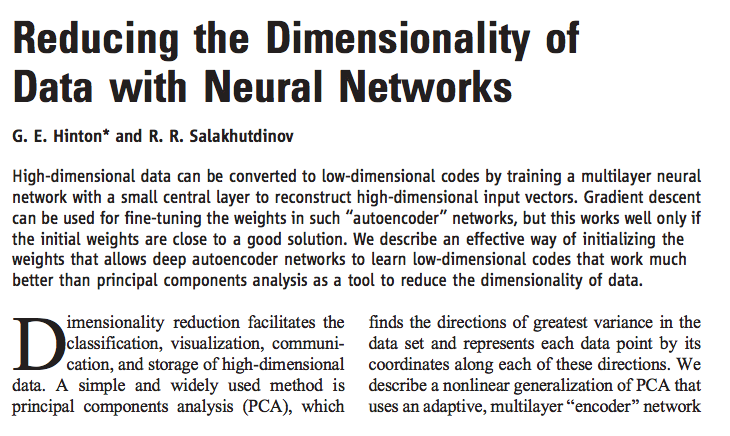
\includegraphics[width=0.95\linewidth]{breakthrough}
	\end{figure}
\end{frame}

\section{Neural Network}

\begin{frame}
	\frametitle{History of Neural Networks}
\begin{itemize}
	\item The 1940s: The Beginning of Neural Networks
\item The 1950s and 1960s: The First Golden Age of
Neural Networks
\item The 1970s: The Quiet Years
\item The 1980s: Renewed Enthusiasm
\end{itemize}
\end{frame}

\begin{frame}
	\frametitle{A Neuron Model}
	\begin{figure}
		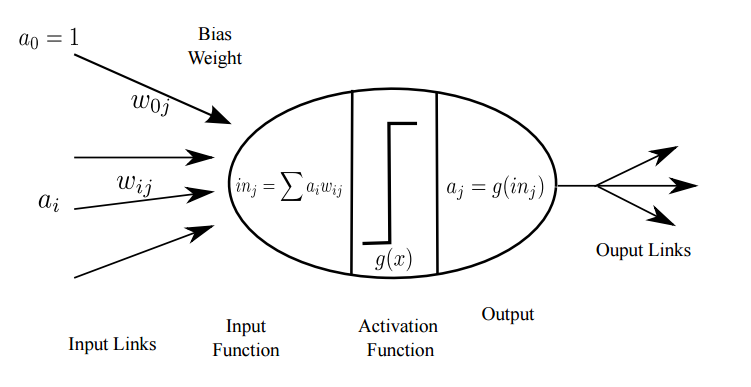
\includegraphics[width=\linewidth]{neuron_model.png}
	\end{figure}
\end{frame}

\begin{frame}
	\frametitle{A Neuron Model}
\begin{itemize}
	\item The weights of the neuron are the parameters of the model.
	\item The input is computed as a weighted sum of the inputs.
	\item The activation function determines the output and can be different functions.
	\item The output is obtained by applying the activation function to the input.
	\item How does the neuron work?
\end{itemize}
\end{frame}

\begin{frame}
	\frametitle{A Neuron Model}
	\begin{figure}
		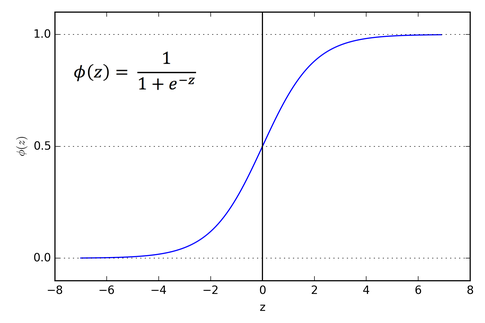
\includegraphics[width=0.8\linewidth]{sigmoid.png}
	\end{figure}
\end{frame}

\begin{frame}
	\frametitle{Single-layer Neural Network}
	\begin{figure}
		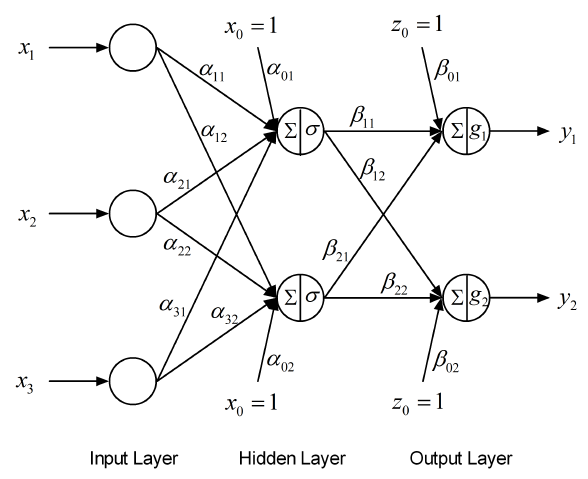
\includegraphics[width=0.8\linewidth]{singlelayer_network1.png}
	\end{figure}
\end{frame}

\begin{frame}
	\frametitle{Multiple-layer Neural Network}
	\begin{figure}
		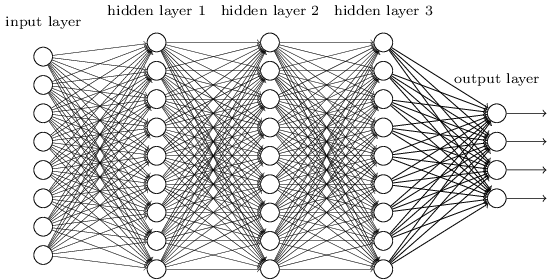
\includegraphics[width=0.8\linewidth]{multilayer_network.png}
	\end{figure}
\end{frame}

\begin{frame}
	\frametitle{Delta Learning Rule}
\begin{itemize}
	\item Based on gradient descent algorithm.
	\item Only applicable for continuous activation function.
	\item The learning signal r is called delta and defined as:
	\begin{equation*}
	r = \{d_{j} - f(\bm{W}_{j}^{T}\bm{X})\}f'(\bm{W}_{j}^{T}\bm{X}) \approx (d_{j}-o_{j})f'(\text{net}_{j})
	\end{equation*}
	\item The weights will be adjusted as:
	\begin{equation*}
	\Delta \bm{W}_{j} = \eta(d_{j} - o_{j})f'(\text{net}_{j})\bm{X}
	\end{equation*}
	
\end{itemize}
\end{frame}

\begin{frame}
	\frametitle{Backpropagation Algorithm}
	\begin{itemize}
		\item BP algorithm is a process of training a neural network
		\item Based on delta learning rule
	\end{itemize}
	\begin{figure}
		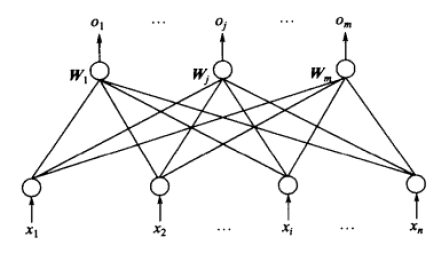
\includegraphics[width=0.8\linewidth]{singlelayer_network.png}
	\end{figure}
\end{frame}

\begin{frame}
	\frametitle{Backpropagation Algorithm}
	The flow of signal in BP algorithm:
	\begin{figure}
		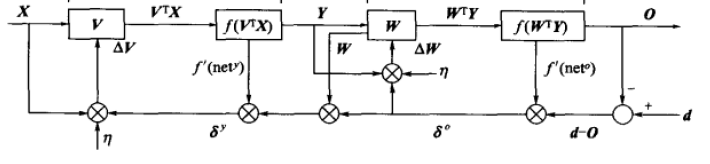
\includegraphics[width=\linewidth]{bp_flow.png}
	\end{figure}
\end{frame}



\section{Convolutional Neural Network}
\begin{frame}
\frametitle{CNN}
\begin{itemize}
	\item Fully connected neural network can bring us too many parameters.
	\item Some patterns are much smaller than the whole image.
\end{itemize}

\begin{figure}
	\hfill
\subfigure{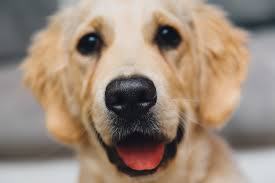
\includegraphics[width=.65\linewidth]{dog1.jpg}}
\hfill
\subfigure{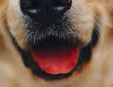
\includegraphics[width=.2\linewidth]{dog2}}
\hfill
\end{figure}

\end{frame}


\begin{frame}
	\frametitle{CNN}
The same pattern appears in different regions.
	
	\begin{figure}
		\hfill
		\subfigure{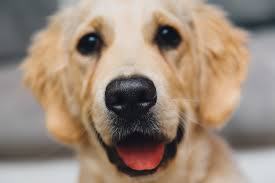
\includegraphics[width=.49\linewidth]{dog1.jpg}}
		\hfill
		\subfigure{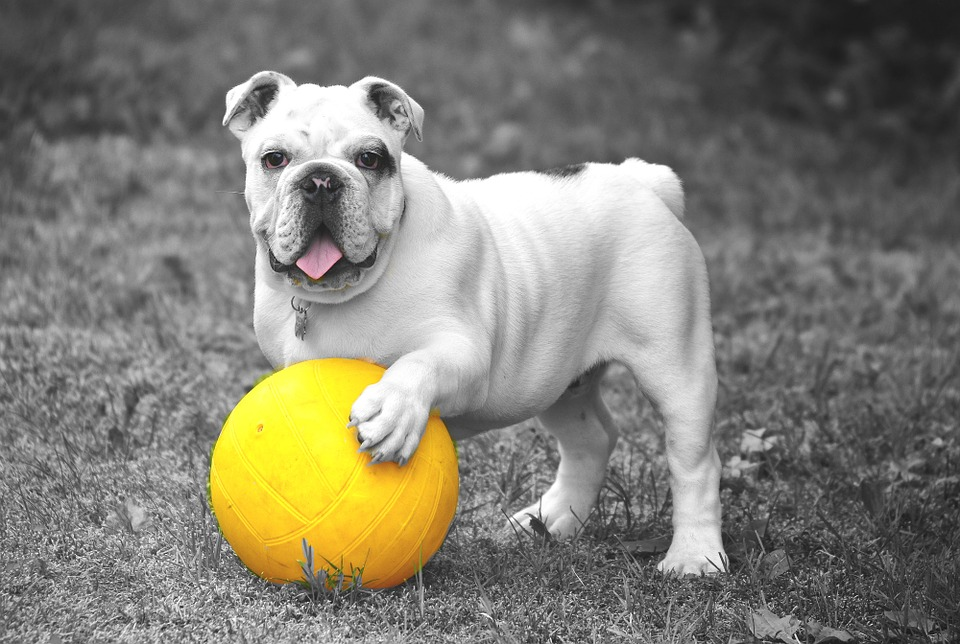
\includegraphics[width=.485\linewidth]{dog3}}
		\hfill
	\end{figure}
	
\end{frame}

\begin{frame}
	\frametitle{CNN}
	The same pattern appears in different regions.
	
	\begin{figure}
		\hfill
		\subfigure{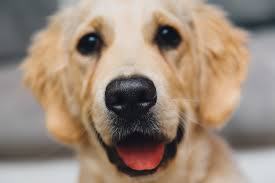
\includegraphics[width=.6\linewidth]{dog1.jpg}}
		\hfill
		\subfigure{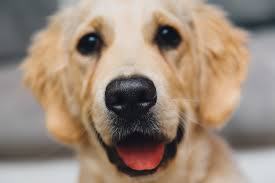
\includegraphics[width=.3\linewidth]{dog1.jpg}}
		\hfill
	\end{figure}
	
\end{frame}

\begin{frame}
	\frametitle{How does convolution work?}
	\begin{figure}
	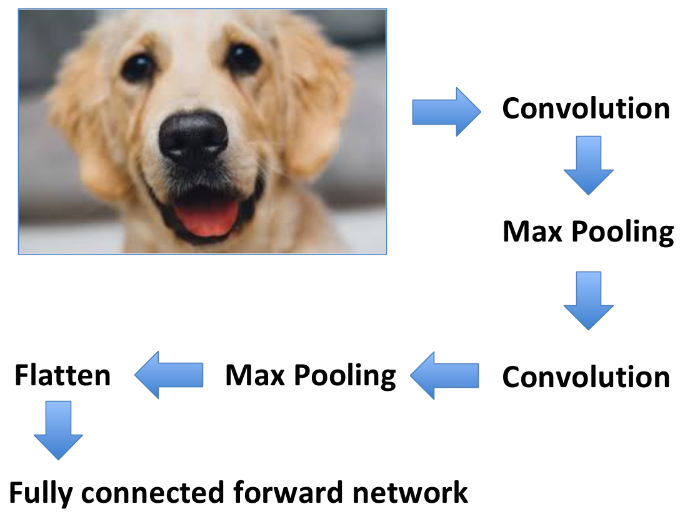
\includegraphics[width=0.9\linewidth]{dog_flow}
	\end{figure}
\end{frame}

\begin{frame}
	\frametitle{How does convolution work?}
	\begin{figure}
		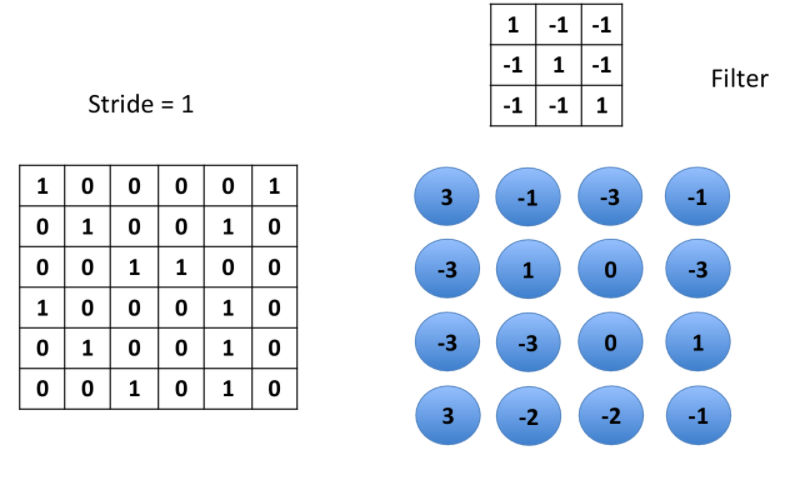
\includegraphics[width=0.9\linewidth]{cnn_procedure_1}
	\end{figure}
\end{frame}

\begin{frame}
	\frametitle{How does convolution work?}
	\begin{figure}
		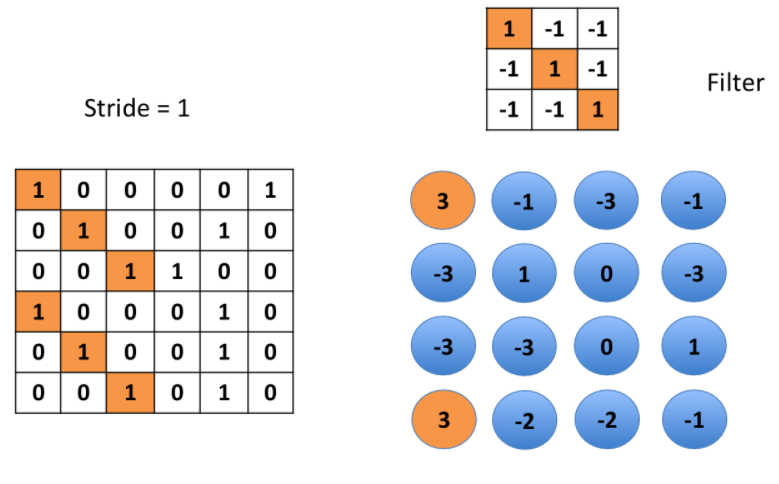
\includegraphics[width=0.9\linewidth]{cnn_procedure_2}
	\end{figure}
\end{frame}

\begin{frame}
	\frametitle{How does convolution work?}
	\begin{figure}
		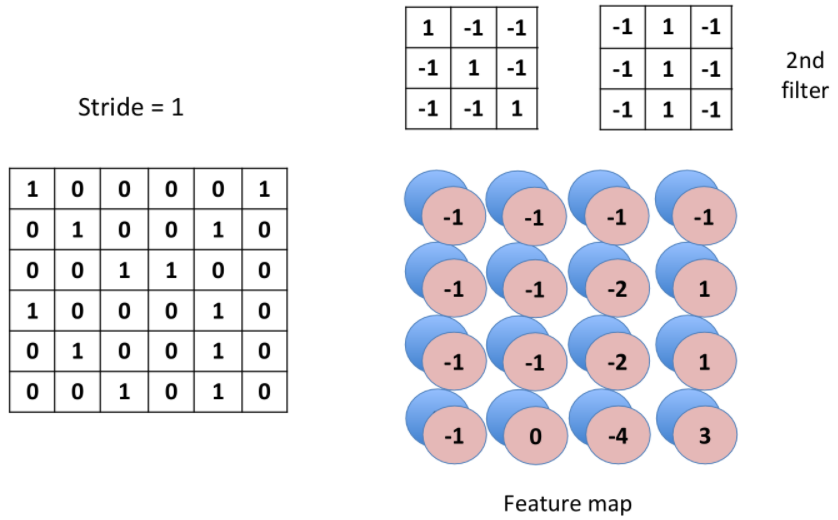
\includegraphics[width=0.9\linewidth]{cnn_procedure_3}
	\end{figure}
\end{frame}

\begin{frame}
	\frametitle{Connection between CNN and Fully Connected Neural Network}
	\begin{figure}
		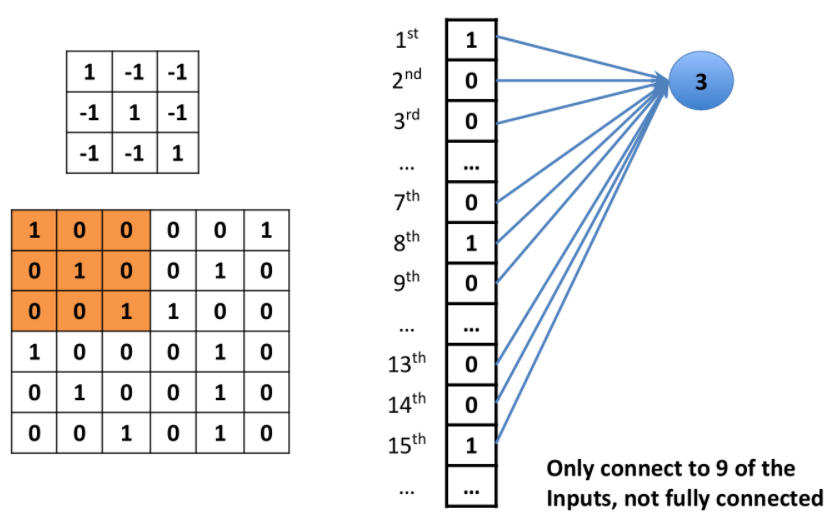
\includegraphics[width=0.9\linewidth]{cnn_procedure_4}
	\end{figure}
\end{frame}

\begin{frame}
	\frametitle{Connection between CNN and Fully Connected Neural Network}
	\begin{figure}
		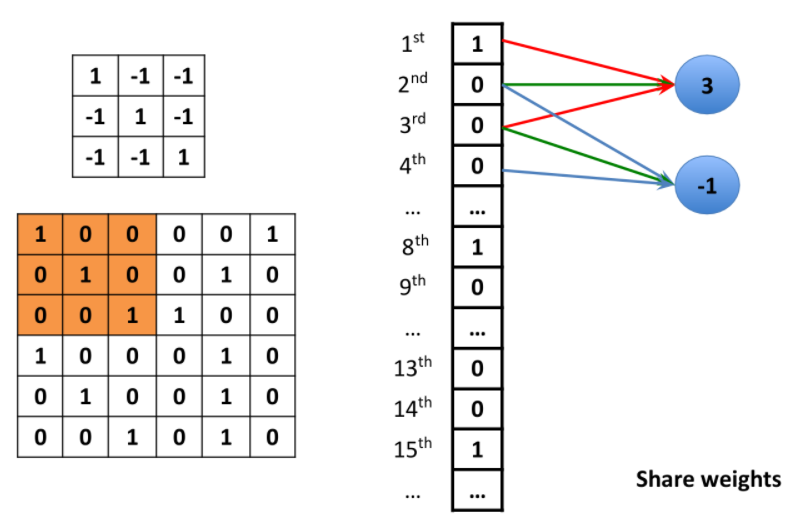
\includegraphics[width=0.9\linewidth]{cnn_procedure_5}
	\end{figure}
\end{frame}

\begin{frame}
	\frametitle{How does max pooling work?}
	\begin{figure}
		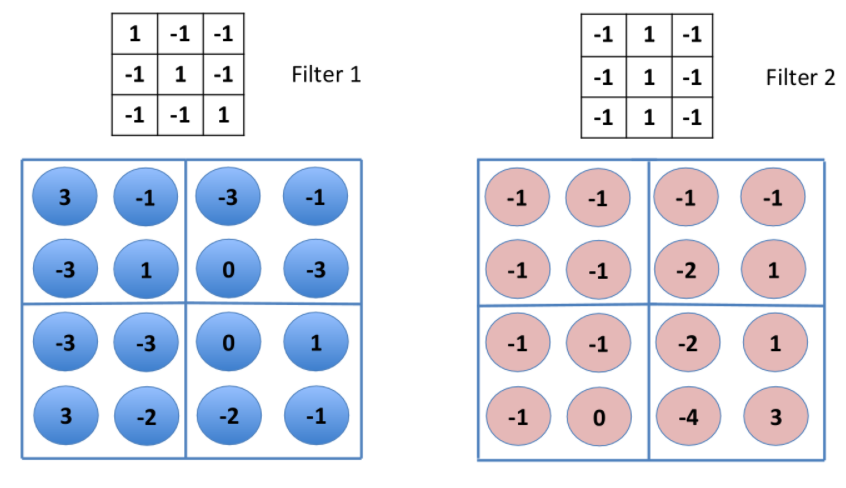
\includegraphics[width=0.9\linewidth]{cnn_procedure_6}
	\end{figure}
\end{frame}

\begin{frame}
	\frametitle{How does max pooling work?}
	\begin{figure}
		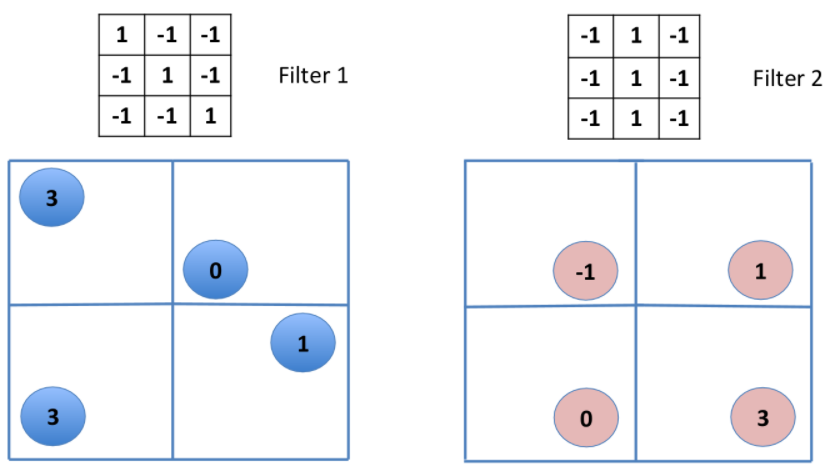
\includegraphics[width=0.95\linewidth]{cnn_procedure_7}
	\end{figure}
\end{frame}

\begin{frame}
	\frametitle{After convolution and max pooling}
	\begin{figure}
		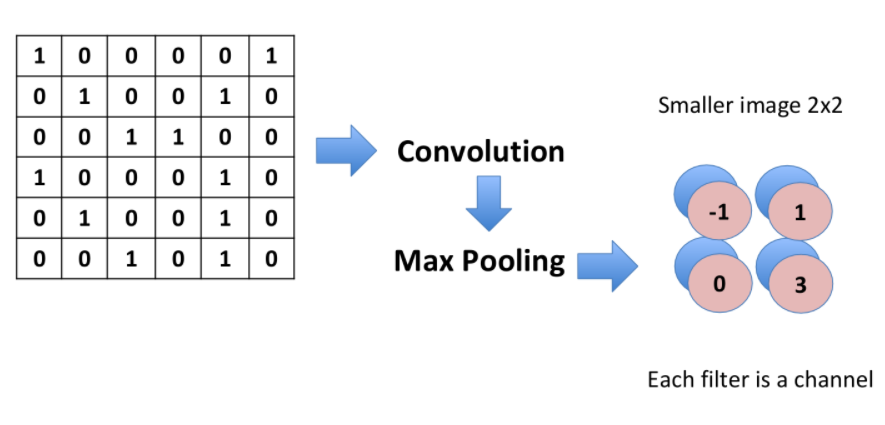
\includegraphics[width=\linewidth]{cnn_procedure_8}
	\end{figure}
\end{frame}

\section{TensorFlow}
\begin{frame}[fragile]{Lists}
Items
\begin{easylist}[itemize]
@ Milk
@ Eggs
@ Potatos
\end{easylist}

Enumerations
\begin{enumerate}
\item First, \item Second and \item Last.
\end{enumerate}

Descriptions
\begin{description}
\item[PowerPoint] Meeh. \item[Beamer] Yeeeha.
\end{description}
\end{frame}

\begin{frame}[fragile]{Tables}
\begin{table}
\caption{Largest cities in the world (source: Wikipedia)}
\begin{tabular}{lr}
\toprule
City & Population\\
\midrule
Mexico City & 20,116,842\\
Shanghai & 19,210,000\\
Peking & 15,796,450\\
Istanbul & 14,160,467\\
\bottomrule
\end{tabular}
\end{table}
\end{frame}

\begin{frame}{Blocks}
Three different block environments are pre-defined and may be styled with an
optional background color.

%   Color Box: Light Orange
\setbeamercolor{boxsthlmLightOrange}{bg=white,fg=pblue}
\begin{beamercolorbox}[wd=\linewidth,ht=10ex,dp=3ex]{boxsthlmLightOrange}
\centering
\texttt{Light Orange}\\
\vspace{1em}
\tiny{RGB:  255,215,210} \\
\tiny{hex: \#ffd7d2}
\end{beamercolorbox}
\end{frame}

\begin{frame}[fragile]{code}
\begin{lstlisting}[language=JavaScript, caption=My Javascript Example]
function someReducer(state = initialState, action) {
  switch (action.type) {
  case 'FOO':
    return Object.assign({}, state, {
      foo: action.payload.foo
    });
  default:
    return state;
  }
}
\end{lstlisting}
\end{frame}

\end{document}
